\section{Workload generation}
In order to simulate different usage cases, a workload generator
has been implemented in the file \emph{wl\_generator.m}, in a similar manner as it was done in the 1st lab session.

This MatLab function takes as parameters a character representing the type of desired distribution, the distribution parameters and the number of samples to generate:

\begin{description}
\item[c:] Constant distribution, i.e. a vector which all elements set to the same value is generated.
\item[b:] Bimodal distribution. Two normally-distributed vectors of the same length are generated using \emph{normrnd}, using different means and variations. Then, the vectors are randomly shuffled together and the result is truncated to the desired length.
\item[u:] Uniform distribution. A vector of data between $u_a$ and $u_b$ is generates using \emph{rand}.
\end{description}


\begin{center}
\begin{figure}[h]
\centering
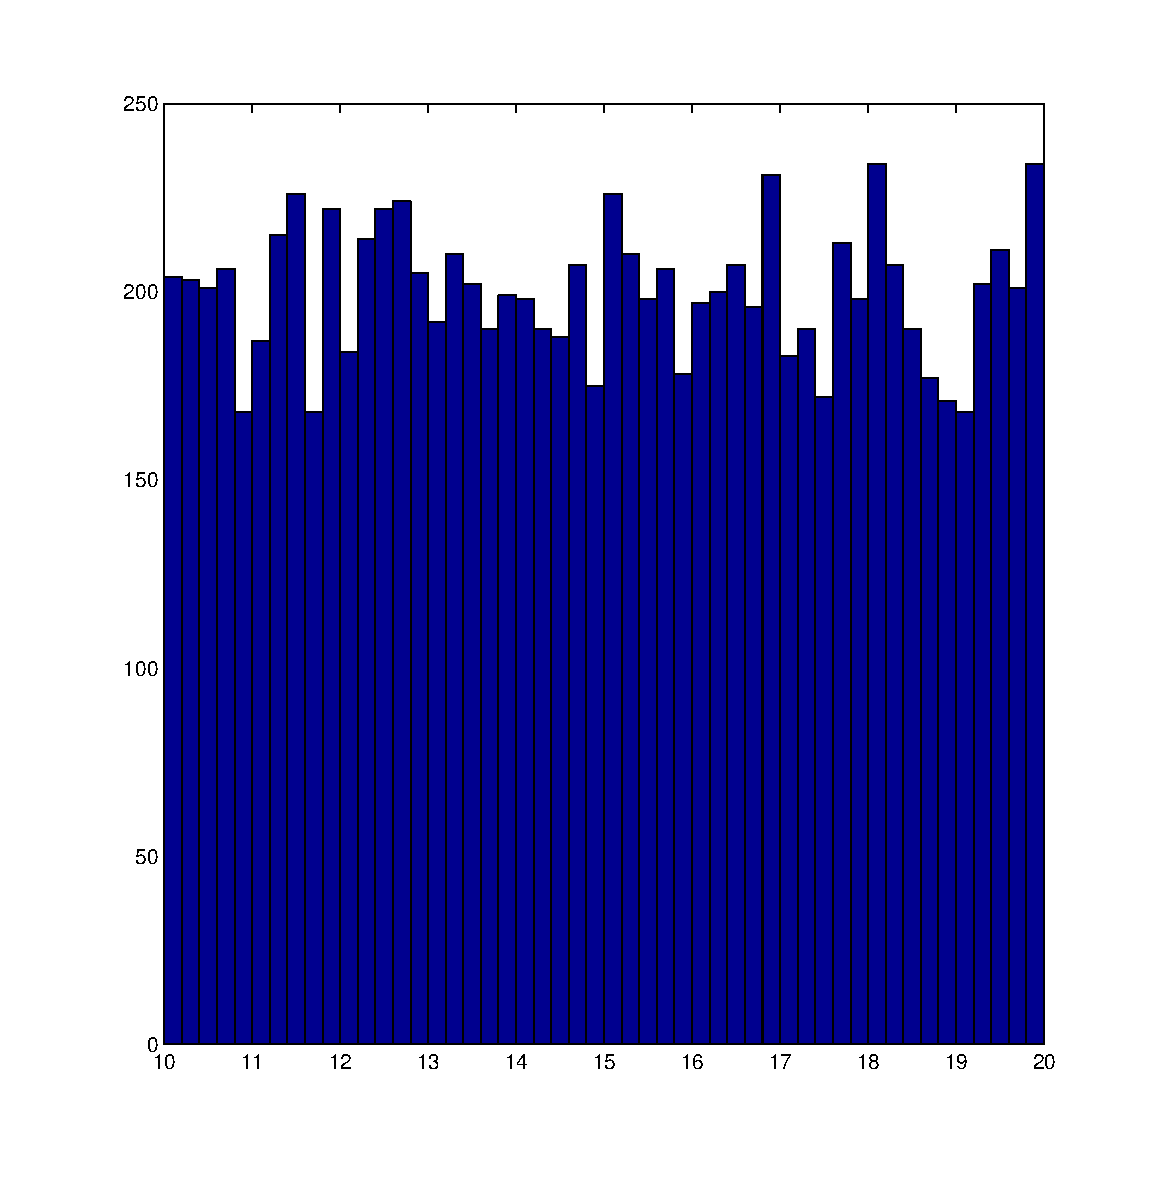
\includegraphics[width=1.5in]{uniform}
%\end{figure} 
%\begin{figure}[h]
%\centering
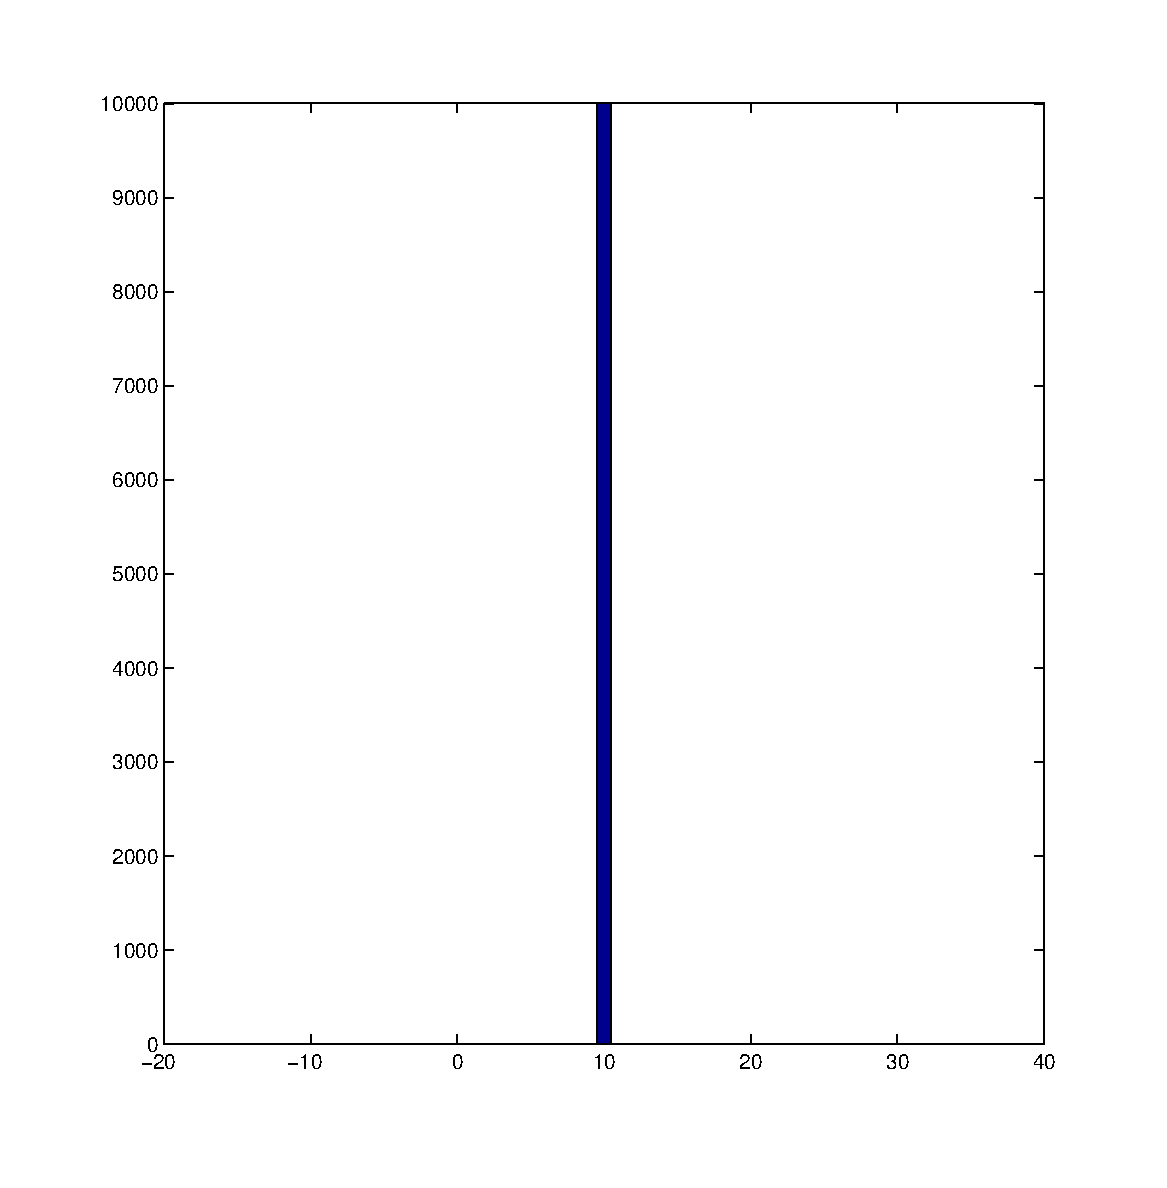
\includegraphics[width=1.5in]{constant}
%\caption{Constant distribution of 10000 values set to 10}
%\end{figure}
%\begin{figure}[h]
%\centering
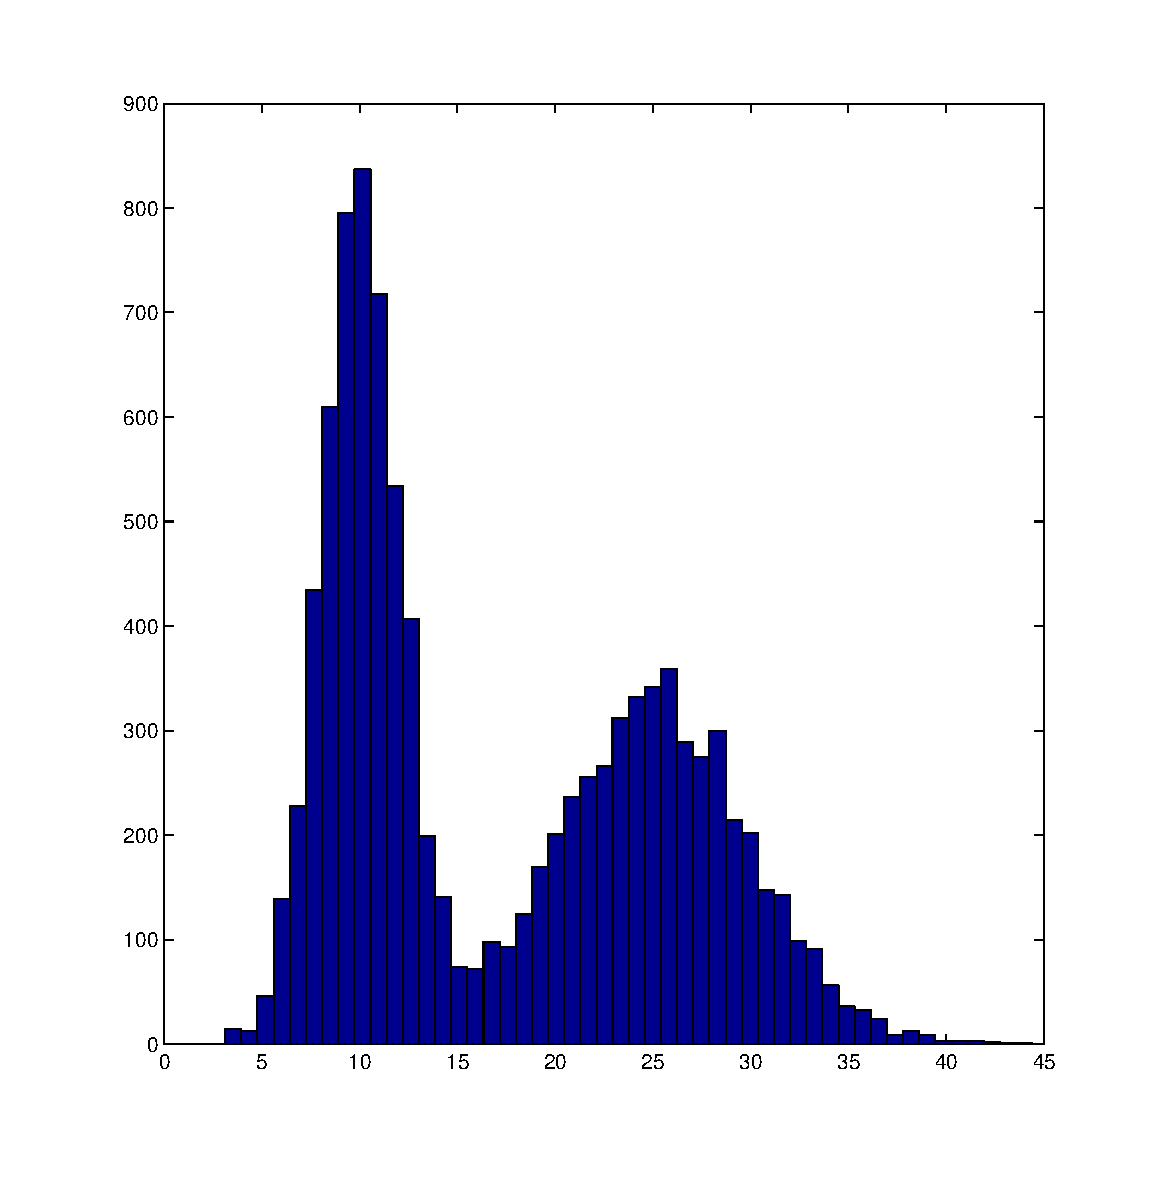
\includegraphics[width=1.5in]{bimodal}
\caption{Random distributions made of 10000 values.\\ Case 1: uniform distribution in range [10, 20];\\ Case 2: constant distribution with value 10;\\ Case 3: bimodal distribution with means 10 and 25 and deviations 2 and 5.}
%\caption{Bimodal distribution of 10000 values with means 10 and 25, and deviations 2 and 5}
\end{figure}
\end{center}

